\documentclass{article}

% Recommended, but optional, packages for figures and better typesetting:
\usepackage{microtype}
\usepackage{graphicx}
\usepackage{subfigure}
\usepackage{booktabs} % for professional tables

% hyperref makes hyperlinks in the resulting PDF.
% If your build breaks (sometimes temporarily if a hyperlink spans a page)
% please comment out the following usepackage line and replace
% \usepackage{icml2021} with \usepackage[nohyperref]{icml2021} above.
\usepackage{hyperref}
\usepackage{xr}
\externaldocument{blind_denoising_SI}
% Attempt to make hyperref and algorithmic work together better:
\newcommand{\theHalgorithm}{\arabic{algorithm}}

% Use the following line for the initial blind version submitted for review:
\usepackage{icml2021}

% custom packages
\usepackage{amsmath}
\usepackage{amssymb}
% for referencing footnotes several times. to load after hyperref
\usepackage{cleveref}
\crefformat{footnote}{#2\footnotemark[#1]#3}
% \usepackage{times}
% \usepackage{epsfig}
% If accepted, instead use the following line for the camera-ready submission:
%\usepackage[accepted]{icml2021}

% The \icmltitle you define below is probably too long as a header.
% Therefore, a short form for the running title is supplied here:
\icmltitlerunning{Joint self-supervised blind denoising and noise estimation}

\begin{document}

\twocolumn[
\icmltitle{Joint self-supervised blind denoising and noise estimation}

% It is OKAY to include author information, even for blind
% submissions: the style file will automatically remove it for you
% unless you've provided the [accepted] option to the icml2021
% package.

% List of affiliations: The first argument should be a (short)
% identifier you will use later to specify author affiliations
% Academic affiliations should list Department, University, City, Region, Country
% Industry affiliations should list Company, City, Region, Country

% You can specify symbols, otherwise they are numbered in order.
% Ideally, you should not use this facility. Affiliations will be numbered
% in order of appearance and this is the preferred way.
\icmlsetsymbol{equal}{*}

\begin{icmlauthorlist}
\icmlauthor{Jean Ollion}{sabilab}
\icmlauthor{Charles Ollion}{cmap}
\icmlauthor{\'Elisabeth Gassiat}{ups}
\icmlauthor{Sylvain Le Corff}{tsp,cmap}
\icmlauthor{Luc Leh\'ericy}{uca}
\end{icmlauthorlist}

\icmlaffiliation{sabilab}{SABILab, Die, France}
\icmlaffiliation{cmap}{CMAP, Ecole Polytechnique, Institut Polytechnique de Paris, France}
\icmlaffiliation{tsp}{Samovar, T\'el\'ecom SudParis, D\'epartement CITI, Institut Polyechnique de Paris, France}
\icmlaffiliation{ups}{Universit\'e Paris-Saclay, CNRS, Laboratoire de math\'ematiques d'Orsay, 91405, Orsay, France}
\icmlaffiliation{uca}{Laboratoire J. A. Dieudonn\'e, Universit\'e C\^ote d'Azur, CNRS, 06108, Nice, France}

\icmlcorrespondingauthor{Jean Ollion}{jean.ollion@polytechnique.org}
\icmlcorrespondingauthor{Sylvain Le Corff}{sylvain.le_corff@telecom-sudparis.eu}

% You may provide any keywords that you
% find helpful for describing your paper; these are used to populate
% the "keywords" metadata in the PDF but will not be shown in the document
\icmlkeywords{Blind Denoising, Self-supervised, Bio-image, Machine Learning}

\vskip 0.3in
]

% this must go after the closing bracket ] following \twocolumn[ ...

% This command actually creates the footnote in the first column
% listing the affiliations and the copyright notice.
% The command takes one argument, which is text to display at the start of the footnote.
% The \icmlEqualContribution command is standard text for equal contribution.
% Remove it (just {}) if you do not need this facility.

\printAffiliationsAndNotice{}  % leave blank if no need to mention equal contribution
% \printAffiliationsAndNotice{\icmlEqualContribution} % otherwise use the standard text.


%%%%%%%%% ABSTRACT
\begin{abstract}
We propose a novel self-supervised image blind denoising approach in which two neural networks jointly predict the clean signal and infer the noise distribution.
Assuming that the noisy observations are independent conditionally to the signal, the networks can be jointly trained without clean training data. Therefore, our approach is particularly relevant for biomedical image denoising where the noise is difficult to model precisely and clean training data are usually unavailable.

Our method significantly outperforms current state-of-the-art self-supervised blind denoising algorithms, on six publicly available biomedical image datasets. We also show empirically with synthetic noisy data that our model captures the noise distribution efficiently. Finally, the described framework is simple, lightweight and computationally efficient, making it useful in practical cases.
\end{abstract}

\section{Introduction}
\label{sec:introduction}

Image denoising is the process of recovering a clean signal $X$ given an observation $Y$ corrupted by a noise $\varepsilon$. Classical denoising approaches  are model-driven in the sense that they rely on strong assumptions on the noise distribution or on the structure of the signal but are often  limited by the relevance of these assumptions.
Recently, efficient data-driven methods have emerged. Most of them assume that pairs made of noisy data $Y$ associated with a clean signal $X$ are available in a supervised learning framework, see for instance \cite{weigert2017content}. In \cite{lehtinen2018noise2noise}, the authors have demonstrated that it is possible to train an efficient denoising method using only pairs of independent noisy measurements $(Y^1, Y^2)$ of the same signal. Such assumptions have also been used to solve deconvolution problem with repeated measurements as in \cite{delaigle2008deconvolution}. However, obtaining  independent observations of the same signal is often unrealistic in practice.

Recent self-supervised methods have overcome this limitation \cite{batson2019noise2self,krull2018noise2void} by training a neural network to predict the value of a (corrupted) pixel value $Y$ only using the noisy observations of the surrounding pixels. In such frameworks, the trained network extracts some local structure in the signal and therefore can be used as a denoiser. Such approaches are referred to as \textit{blind-denoising}  and only assume that the noises associated with different observations are independent and centered. This is well suited to typical microscopy settings, in which both the clean image is unavailable, and the real noise process is complex and not known.

In this paper, we introduce a novel self-supervised method, based on the joint training of two neural networks referred to as D-net (denoiser net) and N-net (noise net). Similar to previous works, the denoiser is a convolutional neural network and receives a masked input during training. Our main contribution is to add the flexible N-net
%which can remove the need to have strong assumptions on the noise distribution: our only assumption is that the noise components associated with the different observations are independent and centered.
%This N-net
which recovers precisely the noise distribution during training, even for complex asymetric noises. We derive this method from a novel mathematical modeling of the denoising problem, opening new avenues for better understanding of why self-supervised networks achieve remarkable results.

The contribution of this paper can be summarized as follows.
\begin{itemize}
  \item We introduce a novel blind denoising model, modeling both the signal and noise distributions.
  \item The proposed architectures outperform state-of-the-art algorithms  over 6 standard microscopy datasets.
  \item We show that N-net recovers the noise distribution efficiently in varying experiments with synthetic noises.
  \item We introduce a novel sharpness metric useful to assess blind denoising quality.
\end{itemize}

\section{Related work}
\label{sec:related}
\paragraph{Denoising by masking observed data.}
Self-supervised denoising methods were introduced by Noise2Void (N2V) \cite{krull2018noise2void} and Noise2Self (N2S) \cite{batson2019noise2self}. They rely on training a function $f_\theta$ depending on an unknown parameter $\theta$, usually  implemented as a convolutional neural network such as the U-net, through masked self-supervision, minimizing the following objective:

$$\mathcal{L}: \theta\mapsto \frac{1}{M}\sum_{i=1}^M \|f_\theta(Y^{masked}_i) - Y_i\|^2\,, $$
where $Y^{masked}_i$ is the image in which the pixel $Y_i$  on which the loss is computed  has been masked. This masking step is crucial to foster learning of  local structure in the signal to predict the masked values.

In practice, the masking procedure has a strong impact on training, as only masked pixels are used for training (typically representing a few percent of the image). In N2V, $\{(Y^{masked}_i,Y_i)\}_{1\leqslant i\leqslant M}$ are sampled  randomly in the picture, and masking consists in replacing $Y_i$ by a random observed value in its neighborhood (with a positive probability of replacing $Y_i$ by itself meaning that no masking is introduced). In N2S,  $\{(Y^{masked}_i,Y_i)\}_{1\leqslant i\leqslant M}$ are obtained with  a fixed grid, and $Y_i$ is replaced by the average of neighboring observations.
%Even though the prediction of a noisy pixel conditionnally on its neighbors is an impossible task to learn perfectly, the estimated function $f_{\hat \theta}$ shows strong denoising properties.
In both cases, the estimated function $f_{\theta}$ shows strong denoising properties.

These methods however suffer from high frequency denoising artifacts known as \textit{checkerboard pattern}. Finally, \cite{broaddus2020removing} showed that when the noise has  local correlations (for instance a  directional noise), the masking can be adapted (by masking adjacent pixel in the same direction as the noise spatial correlation for instance) to remove them. These works have been extended in DecoNoising \cite{goncharova2020} in which a Gaussian convolution is added after the neural network output to simulate microscope Point Spread Function. This technique improves performances, however the deconvolved image (predicted image before the Gaussian convolution) has even stronger checkerboard pattern.

\paragraph{J-invariant networks.}
Learning to predict a collection of held-out pixels of an image, from all the other pixels and masked versions (as in N2V, N2S) can fit in the J-invariant framework introduced by \cite{batson2019noise2self}.
A J-invariant function does not depend on a few selected dimensions J of its input variables; typically a few masked pixels
in the picture.
This usually translates in this function being a convolutional function which does not depend on the central pixel, but rather on all the observations in its neighborhood. Those functions are sometimes also called \textit{blind spot}.
% This independance guarantees that such a function learnt through self-supervision is not the identity.
 Additionally, \cite{batson2019noise2self} also provided theoretical guarantees that a J-invariant function may seperate noise from signal and produce near-optimal denoisers.

However, in practice, Neither N2V nor N2S use strictly J-invariant functions, as they remove the masks at inference time,
effectively using all the pixels, resulting in significantly better performance. By having this difference between train and test time, it is not well understood how the denoiser uses the central pixel information, as it was not seen during training. The performance boost might be due to the inductive bias of the convolutional architecture, but understanding further this dependency could lead to better performances.
Few other works have true J-invariant functions which are kept J-invariant at test time, however this is not trivially achieved in convolutional neural networks. This was achieved in \cite{laine2019high} by introducing directional convolution kernels, which only depend on pixels in specific directions, ensuring that the value does not depend on pixels on the opposite direction. The function is therefore J-invariant, where J is a partition of the image, excluding the central pixel, depending on the direction chosen. One drawback is that the inference has to be performed four times, in each direction.
More recently, \cite{lee2020noise2kernel} introduced a combination of specific convolution operators with dilation and strides, ensuring that the function is independent of the central pixel by design, therefore J-invariant with J being the center pixel. This also benefits the training procedure, as it does not require a tuned masking procedure. However, this constrains strongly the network architecture, and the reported results are less competitive than alternative methods.

\paragraph{Contribution of a noise model.}
The denoising literature includes few works which explicitely model the noise distribution. In \cite{laine2019high}, the authors used Gaussian noise independent of the signal and Poisson-Gaussian noise, i.e. a Gaussian noise with variance scaling linearly with the signal value, as well as impulse noise, i.e. a uniform noise.
In this work, the noise parameters are either known or estimated with an auxiliary neural network.
As the signal distribution and the noise distribution belong to a known parametric family, the central pixel can be included at test time in order to improve performances.
%This is only possible because a truly J-invariant function is used at test time.
This approach is consistent and yields good results, but is then restricted to known, synthetic noise distributions and therefore falls under the category of \textit{non-blind denoising} methods.

In \cite{krull2019probabilistic,prakash2020fully,2020DivNoising}, make use of a noise model, which is a more generic modelisation of the ditribution of the noise given the signal intensity: $p(y|x) = N(x): \mathbb{R} \to \mathbb{R}$, and can better model real noises.
In these works, noise models are approximated using 2D histograms of denoised and noisy observed values, either using additional calibration data \cite{krull2019probabilistic} (in that case the method is not fully self-supervised) or using a previously trained denoising function \cite{prakash2020fully}. In one variant, the noise distribution is fitted with gaussian mixture model with empirically designed constrains.
The denoising network is then trained to predict a whole histogram distribution of possible noisy values, approximating the previously defined noise distribution at each pixel.
This rather inefficient as it requires to predict $800$ values instead of a single point estimate of each pixel.
Both methods can improve performances but still display a checkerboard pattern and sometimes produce numeric instabilities during training \cite{goncharova2020}.
The result also depends on the binning choice made to build the 2D histogram, which is not trivial in the case of fluorescence-microscopy data where signal range can be very high.
Their complexity is higher than N2V/N2S as they require $2$ training procedure and callibration data or $3$ training procedures.
Finally, \cite{2020DivNoising} uses the Variational Autoencoder formalism, adding a pre-calibrated noise model in their architecture.
This method yeilds rather blurry images and sometimes generates hallucination artefacts.

It is worth noting that supervised \textit{blind denoising} methods have used parametrized noise model, such as \cite{zhang2017beyond,yue2019variational}, which explicitely uses large neural networks to model a complex noise, with even less assumption on the noise (noise can be slightly structured, not centered...). Even though \cite{yue2019variational} is able to train jointly a noise network and a denoiser, their modeling only works in a supervised setting, which it does not apply in our setting.

The work of Laine et al. \cite{laine2019high} gives the intuition that a striclty J-invariant function lacks the information of the central pixel at test-time.
On the contray, methods such as N2V or N2S use the central pixel at test-time, but the dependency on central pixel is not explicit and unknown.
Instead of focusing on finding new strictly J-invariant functions, our approch rather focuses on having efficient masking procedure only at train-time.
We provide a few directions to explain why relaxing the J-invariance might be beneficial.
This also gives the flexibility to tune the masking to match structured noise, which we observed in 2 of the 6 datasets (see section X) \cite{broaddus2020removing}.

\section{Model}
\label{sec:model}

Estimating a signal corrupted by additive noise  is a challenging statistical problem. In such frameworks, the received observation $Y$ is given by $Y = X + \varepsilon$,  where $X$ is the signal and $\varepsilon$ is the noise. A lot of works have been devoted to deconvolution where the aim is to recover the distribution of the signal based on the observations. It has been for instance applied in a large variety of disciplines and has stimulated a great research interest in signal processing \cite{moulines1997maximum,attias1998blind}, in image reconstruction \cite{kundur1996blind,campisi2017blind}, see also  \cite{meister:2009}.


Recently, \cite{gassiat:lecorff:lehericy:2021} proved that it is possible to recover the signal distribution when $X$ has at least two dimensions and may be decomposed into two subsets of random variables which satisfy some weak dependency assumption. This identifiability result does not require any assumption on the noise distribution but illustrates that the components of the signal must be dependent to allow its identification. %The results proposed in \cite{gassiat:lecorff:lehericy:2021} motivate the denoising approach introduced in this paper where several classes of noises are considered to describe the observations received from the target signal.  %The signal $X$ is modeled as a function of the noisy observation $Y$ and its neighborhood $\Omega_Y$: $X =  \mu_{\theta_p}(\Omega_Y;Y)$.

In this paper, it is assumed that the observation $Y$ associated with $X$  is given by
\begin{equation}
\label{eq:def:Y}
Y = X + \sigma_{\theta_n}(X)\varepsilon\,,
\end{equation}
%which means that
%$$
%Y = X + (\mu_{\theta_p}(\Omega_Y;\overline{\Omega_Y})-\mu_{\theta_p}(\Omega_Y;Y)) + \sigma_{\theta_n}(\mu_{\theta_p}(\Omega_Y;\overline{\Omega_Y}))\varepsilon
%$$
%The blind denoising framework introduced in this paper can be written as a regression problem where the observations conditionally on $\Omega_Y$ the observation is given by
%$$
%Y = \mu_{\theta_p}(\Omega_Y;\overline{\Omega_Y}) + \sigma_{\theta_n}(\mu_{\theta_p}(\Omega_Y;\overline{\Omega_Y}))\varepsilon\,,
%$$
where $\varepsilon$ is a centered noise independent of $X$ and $\sigma^2_{\theta_n}$ is parameterized by a convolutional neural network, called \textit{N-net} and with unknown weights $\theta_n$.
In standard approaches \cite{},  $\varepsilon$ is assumed to be a centered Gaussian random variable and  $\sigma^2_{\theta_n}(\cdot)$ is either known and constant \cite{} or has a Poisson-Gaussian shape i.e., scales with $\alpha X + \eta^2$, see \cite{}.
In \cite{gassiat:lecorff:lehericy:2021}, the signal is assumed to be multivariate with  $\sigma^2_{\theta_n}$ independent of $X$. Model \eqref{eq:def:Y} does not fit directly the assumptions of \cite{gassiat:lecorff:lehericy:2021} and identifiability of the noise and signal  distributions remains an open problem in this setting.
%However, our approach in this paper is motivated by the fact that $\varepsilon$ is independent of $X$ and that $X$ depends on its neighborhood.

%Conditionally to $X$, we propose a more general corrupting process as $\varepsilon$ is a centered Gaussian random variable with variance $\sigma^2_{\theta_n}(X)$ where $\sigma^2_{\theta_n}$ is parameterized by a convolutional neural network, called \textit{N-net} and with unknown weights $\theta_n$.
%We also propose an extension of this setting in which $\varepsilon$ is a mixture of Gaussian random variables with state-dependent variances to account for skewness.
Let  $\Omega_X$ be the signal values in a neighborhood of $X$.
In this paper, we assume that $(X,\Omega_X)$ is a random vector with dependent variables and propose to model the conditional mean of $X$ given $(Y,\Omega_Y)$ by a parametric function denoted by $\mu_{\theta_d}$ so that $\mathbb{E}[X|Y,\Omega_Y] = \mu_{\theta_d}(\Omega_Y,Y)$ where $\Omega_Y$ are the noisy observations of the signals in the neighborhood of $X$. The function $ \mu_{\theta_d}$ is parameterized by a convolutional neural network, called \textit{D-net} and with unknown weights $\theta_d$.

A natural estimator of $X$ given the noisy observations is given by $\widehat X = \mu_{\theta_d}(\Omega_Y,Y)$. During training this predictor $\widehat X$ cannot be used to estimate $\theta_d$ and $\theta_n$ as  a standard mean squared error loss would recover the prediction of $Y$ instead of $X$. This is the reason why we adopt a blind spot denoising approach and assume during training that $\mu_{\theta_d}$ cannot use $Y$ as an input which must be replaced by an estimator. In this framework, an appealing prediction of $Y$ is given by $\mathbb{E}[Y|\Omega_Y]$ which we estimate by $\mu_{\theta_d}(\Omega_Y,g(\Omega_Y))$ where $g$ is a known function. In the experiments below, we chose to set $g(\Omega_Y)$ as the empirical mean of the noisy pixels in $\Omega_Y$.

%The signal $X$ is then modeled as
%\begin{equation}
%\label{eq:def:X}
%X =  \mu_{\theta_p}(\Omega_X,U)\,,
%\end{equation}
%where $\Omega_X$ are the signal values in a neighborhood of $X$ and $U$ is a random variable on $\mathbb{R}$. % $\Omega_X$-measurable.
% In the case where the random variable $U$ is $\Omega_X$-measurable, there exists a measurable function $g$ such that $U = g(\Omega_X)$.
Combining this with the additive model  \eqref{eq:def:Y} yields the following loss function associated with $N$ observations $(Y_1,\ldots,Y_N)$:
$$
\ell_{\theta}: (Y_1,\ldots,Y_N) \mapsto \frac{1}{N}\sum_{i=1}^N \ell_{\theta}(Y_i|\Omega_{Y_i})\,,
$$
where $\theta = (\theta_n,\theta_d)$ and
\begin{multline*}
\ell_{\theta}(Y_i|\Omega_{Y_i}) = \frac{1}{2}\log(\sigma_{\theta_n}( \mu_{\theta_d}(\Omega_{Y_i},g(\Omega_{Y_i})))^2) \\
+\frac{1}{2}\left(\frac{Y_i-\mu_{\theta_d}(\Omega_{Y_i},g(\Omega_{Y_i}))}{\sigma_{\theta_n}(\mu_{\theta_d}(\Omega_{Y_i},g(\Omega_{Y_i}))}\right)^2\,. %\frac{(Y_i-\mu_{\theta_p}(\Omega_{Y_i};\overline{\Omega_{Y_i}}))^2}{\sigma_{\theta_n}(\mu_{\theta_p}(\Omega_{Y_i};\overline{\Omega_{Y_i}}))^2} \,,
\end{multline*}
%This loss is obtained by computing the conditional loglikelihood of $Y$ given $X$ evaluated at the predictor of $Y$ obtained by replacing $\Omega_{X}$ by the observed values $\Omega(Y)$ in \eqref{eq:def:X}.
In Section~\ref{sec:experiments} we propose other noise distributions to account for positive skewness which cannot be modeled with Gaussian distributions. We also provide empirical evaluations that choosing $g$ as the empirical mean of its entries is a robust and appealing solution while other choices can be made straightforwardly.
%The random variable $U$ being  $\Omega_X$-measurable, there exists a measurable function $g$ such that $U = g(\Omega_X)$

%After a training phase to estimate $\theta$, the signal values cannot be predicted as the random variable $U$ is not observed. Several predictors of $X$ can be designed.



%uses the fact that by \eqref{eq:def:X} $Y_i$ is a natural linear predictor of $X_i$ and then
%instead of introducing an explicit noise  distribution in the definition of $U$ and  therefore in \eqref{eq:def:X} and then to estimate the posterior distribution of $X$ given $Y$ we propose to introduce a loss function which

% and $\overline{\Omega_Y}$ is the empirical mean of $\Omega_Y$.
%The approach proposed in this paper is decomposed into two steps.
%\begin{enumerate}
%\item First, $\mu_{\theta_p}$ is obtained with the P-Net fed with $\Omega_y$ and $\overline \Omega_y$ at central position, $\sigma_{\theta_n}^2$ is  obtained with the N-Net fed with $\mu_{\theta_p}$.
%\item After a training procedure to estimate the parameters of these networks, the estimator of the unknow pixel given the observations $(y,\Omega_y)$ is set to $\mu_{\theta_p}(\Omega_y,y)$ as an approximation of the posterior mean.
%\end{enumerate}
%The signal $X$ is then modeled as $X =  \mu_{\theta_p}(\Omega_Y;Y)$ so that
%$$
%Y = X + \Delta_{\theta_p}(\Omega_Y;\overline{\Omega_Y},Y) + \sigma_{\theta_n}(\mu_{\theta_p}(\Omega_Y;\overline{\Omega_Y}))\varepsilon\,,
%$$
%where
%\begin{align*}
%\Delta_{\theta_p}(\Omega_Y;\overline{\Omega_Y},Y)  &=  \mu_{\theta_p}(\Omega_Y;\overline{\Omega_Y})  -\mu_{\theta_p}(\Omega_Y;Y) \,,\\
%&\sim \partial_2\mu_{\theta_p}(\Omega_Y;Y)[\overline{\Omega_Y}-Y]
%\end{align*}


\section{Experiments}
\label{sec:experiments}
\subsection{Model Architecture}
\paragraph{D-Net}
The function $\mu_{\theta_d}$ was parameterized by a UNet \cite{ronneberger2015u} deep neural network, which has a fully convolutional architecture.
We propose several changes from the original version: we do not crop the image and use zero-padding instead, we use 2 levels of contractions/expansions with 64 filters, expansions is performed by an upsampling layer with nearest-neighbor approximation directly followed by 2x2 convolution, we added two layers of 1x1 convolution with 64 filters and ReLU activation at the end of the network, and set no activation function at the output layer.
The main difference with the networks used in N2S and N2N is that we use upsampling layer instead of transpose convolution, as we observed transpose convolution tend to increase the checkerboard artefact. This was also observed by \cite{kobayashi2020image}.
The receptive field of this network is 35x35 pixels.
At test-time, we averaged the prediction of the image with the predictions of its transposed and flipped versions on each axis, which improves slightly performances in terms of PSNR and SSIM.
% For natural images, we used 3 levels of contractions/expansions and 128 filters.

% \textit{[Jean] cette section ne devrait-elle pas aller ailleurs ? ou supprimée?}
% This implies that at a given coordinate $(l,m)$, $(\mu_p^{(l,m)}, \sigma_p^{(l,m)})$ depend on $x^{(l,m)}$ and its neighborhood.
% While the central pixel $x^{(l,m)}$ is masked during training (its value is replaced with a deterministic function of the neighboring pixels), the convolutional architecture still uses the replaced value and learns the parameters of the convolution associated with this central value.

\paragraph{N-Net}
The function $\sigma_{\theta_n}$ describing the local variance of the noise distribution is parameterized by a fully convolutional network composed 3 successive blocks, each block being composed of two 1x1 convolutions layers of 64 filters, each followed by a non-linear activation layer (alternatively tanh and leaky ReLU with alpha parameter set to $0.1$).
A convolution 1x1 with a single channel followed by an exponential activation function is placed after the last block.
\textit{TODO: describe architecture in GMM mode. Graphe en SI ? }

This choice is motivated by the fact that such networks can be trained in a supervised way with a clean image $X$ as input and the following cost function, where $Y$ is a corrupted observation of $X$ \textcolor{red}{il faut l'llustrer dans les supplementary non ?}:$y\mapsto\varphi_{0,\sigma_n^2}(x)$.
The essential aspect of the architecture is that the network contain no spatial convolution (only 1x1 convolutions), otherwise the noise distribution is not well described by the network. This is consistent with our model, in which the noise is independent of the neighborhood.

\subsection{Masking procedure}
Following \cite{batson2019noise2self}, we masked pixels along a grid. The loss is computed only on the masked pixels.
We obtained the best results with a replacement by a 3x3 gaussian filter with $\sigma=1$ with a weight equal to zero at the center position, and a sum of weights equal to 1.
The drawback of maksing along a grid is that for a given receptive field, pixels are masked at fixed positions. If grid spacing is too low, then too many masked pixels are present in the receptive field and perturbs the performances, because the network learn to avoid using masked pixels for prediction. On the other hand, the larger the spacing, the less pixels are used for training, which reduces dramatically training efficiency.
In order to push the limits of this trade-off between learning efficiency and denoising quality, we introduced two modifications on the original approach: we used a random dynamic spacing between 3 and 5 pixels, which allow to have relative positions of masked pixels that change randomly.

\subsection{Datasets}
We trained and evaluated our method on 6 publicly available datasets of microscopy images. In those datasets, ground truth is estimated by averaging several observations of the same field-of-view (FOV).

The 3 first datasets have been published along with the PN2V method\cite{krull2019probabilistic}, each is composed of several observations of the same FOV. \emph{Convallaria} dataset, refered to as \emph{PN2V-C} is composed of 100 observations of size $1024$x$1024$; \emph{Mouse skull nuclei} referred to as \emph{PN2V-MN} is composed 200 images of size $512$x$512$ and \emph{Mouse Actin} refered to as \emph{PN2V-MA} is composed of 100 images of size $1024$x$1024$.
To be able to compare our method, we used the same training and evaluation sets as the authors: for each sample type the whole dataset is used for training, and only a subset of the FOV is used for PSNR computation: $(Y,X)\in([0, 512], [0, 512])$ for PN2V-C, $([0, 512], [0, 256])$ for PN2V-MN and $([0, 1024], [0, 512])$ for PN2V-MA.

The 3 last datasets are the 3 channels of the W2S dataset\cite{zhou2020w2s} refered to as \emph{W2S-1}, \emph{W2S-2} and \emph{W2S-3}.
We used the 16-bit raw images kindly provided by the authors.
The dataset is composed of 120 FOV of 400 observations of size $512$x$512$ pixels.
The first 80 are used for training and the last 40 for evaluation.
Following the authors, for each FOV, only the raw image of index 249 is used for training or for evaluation, which corresponds better to most use case where only one observation per FOV is available.

Images were normalized using the modal value as center and the difference between modal value and $95\%$ percentile as scale factor, computed on the whole dataset.\footnote{This is relevant in fluorescence microscopy data where signal is often less abundant than background with proportion that vary among images and siganl distribution has often an heavy tail towards high values.}

\subsection{Training}
Networks are trained using Adam optimizer with a learning rate of $4*10^{-4}$, decreased by $\frac{1}{2}$ on plateau of 30 epochs until $1*10^{-6}$. We trained networks for 400 epochs of 200 steps.
This is an over-estimation of the required training as we observed that networks reach a near-optimal state within the first 100 epochs, but we kept a longer training to have more reproducible results.
We obtained better and more reproductible results using the weights of the trained model at the last epoch instead of the weights of the model with the best validation loss, possibliy because the loss is a bad proxy for the denoising performances. For that reason, we did not use a validation step.
Each batch is composed of (overlapping) random tiles of 96x96 pixels for microscopy datasets.
Batch size was set to 4 for \emph{PN2V-C} and 1 for all other datasets.
Each mini batch was cut into 100 tiles.
Tiles were augmented with random horizontal and/or vertical flip and/or a random rotation with an angle chosen within $(90^\circ, 180^\circ, 270^\circ)$.

We observed that dataset \emph{PN2V-C} and \emph{PN2V-MA} display axial correlation in the noise, for those datasets we adapted the masking produre as in \cite{broaddus2020removing}: the replacement value was computed on a neighborhood excluding the neighbors along the correlation axis, and neighbors were masked on this axis, within an extent of 2 pixel for \emph{PN2V-C} and 3 pixels for \emph{PN2V-MA}.
Those ranges can be determined easily in a self-supervised setup because the neural network tend to amplify the noise correlation, thus one can easily chose the smallest range for which the axial correlation disapears.
Importantly, for those datasets, only data-augmentation is only composed of combinations of flips to avoid axes transposition.

\subsection{Evaluation}
For the 6 chosen datasets, images are encoded in 16-bit thus the actual data range of each ground truth image is used for PSNR computation.
When comparing images, the PSNR is not highly indicative of perceived similarity, in particular it do not reflect similarity of high frequency information such as textures and local contrasts \cite{wang2004image}, that denoising methods tend to reduce. It is thus essential to have other metrics that them into account.
To address this shortcoming, we used Structural similarity (SSIM) that take textures and edges into account \cite{wang2004image}, computed as in the original work.

\section{Results}
\subsection{Noise estimation}

\begin{figure}[ht]
\vskip 0.2in
\begin{center}
\centerline{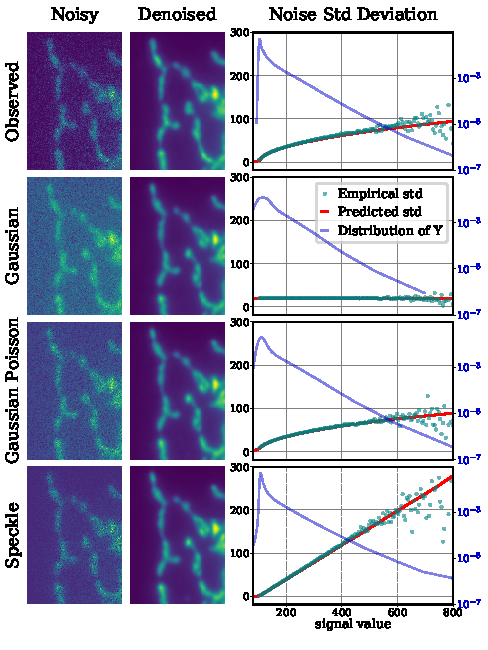
\includegraphics[width=\columnwidth]{fig_noise_std.pdf}}
\caption{Noise estimation.
For 3 models of synthetic noise and the observed noise, the plots display the empirical standard deviation of the noise $Y - X$, as well as the predicted standard deviation of the noise by NNet\footnotemark as a function of $X$.
Theoretical standard deviation of the noise is displayed for the 3 models of synthetic noise.
The empirical ditribution of $Y$ is displayed in blue, in logarithmic scale.
Examples of noisy images and the corresponding predicted denoised images are displayed in columns \textit{Noisy} and \textit{Denoised}.}
\label{fig:noisestd}
\end{center}
\vskip -0.2in
\end{figure}
\footnotetext{Display range was shrinked in Y-axis for visualization purposes, excluding some points of the empirical std of the Speckle noise model.}
To evaluate the capacity of the N-net to capture blindly different noise distributions, we generated 3 datasets by adding synthetic noise to the ground truth of dataset \textit{w2s-1}, and we chose the parameters of the noise models so that PSNR of noisy images match the one of the orignial dataset (in a range of $\pm0.1$dB).
We used 3 classical noise models: additive gaussian, poisson-gaussian and speckle, see Sup.~section~\ref{si:synthetic} for details.
Empirical and predicted distributions of noise standard deviation are illustrated in Fig.~\ref{fig:noisestd}.
It shows our method is able to capture the different noise distributions even in areas where signal is rare.

\subsection{Improving estimation on real noise}
\begin{figure}[ht]
\vskip 0.2in
\begin{center}
\centerline{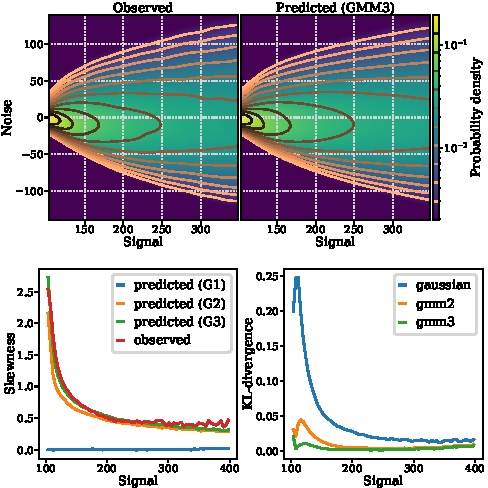
\includegraphics[width=\columnwidth]{fig_skewness.pdf}}
\caption{Real noise estimation. \textbf{Upper-left}: empirical distribution of the noise $Y - X$ as a function of $X$, normalized in each signal value bin\textit{faut il le préciser ou c'est évident?} for dataset \textit{w2s-1}.
\textbf{Upper-right}: corresponding predicted noise distribution for a 3-component-GMM.
\textbf{Lower-left}: Skewness of empirical and predicted noise distribution as a function of $X$, estimated with Pearson's moment coefficient of skewness\footnotemark.
\textbf{Lower-rigth}:  Kullback–Leibler divergence between empirical noise ditribution and predicted ditribution generated by each model, as a function of $X$.
\textit{G1} stands for Gaussian model, \textit{G2} for a 2-component-GMM and \textit{G3} a 3-component-GMM.
}
\label{fig:skewness}
\end{center}
\vskip -0.2in
\end{figure}
\footnotetext{All the graphs are computed using regular signal value bins and excluding signal values greater to the $XX\%$ percentile of the dataset so that there is enough observed samples in each bin to compute statistically significant metrics.}
We observed that contrary to the classical noise models, the observed noise often display a certain degree of skewness, as illustrated in Fig.~\ref{fig:skewness}.
In order to be able to capture this aspect, we predict a Gaussian mixture model (GMM) instead of a simple Gaussian model as described in Section~\ref{sec:model}. Fig.~\ref{fig:skewness} shows that noise skewness is well described by the predicted model, and the noise distribution is better discribed by a GMM than by a single Gaussian.

\subsection{Denoising performances}
\label{sec:perf}
\begin{table*}[t]
\caption{Evaluation of our method on 6 datasets with PSNR/SSIM metrics. SSIM estimate sharpness. Metrics computed on noisy images are displayed in the \textit{Observed} columns. For DecoNoising and N2V, PSNR are taken from \cite{goncharova2020} and SSIM are computed on prediction made by networks trained using the source code provided by the authors\footnotemark. \textit{Gaussian} corresponds to the optimal gaussian baseline defined in section~\ref{sec:perf}.}
\label{table:results}
\vskip 0.15in
\begin{center}
\begin{small}
\begin{sc}
\begin{tabular}{l@{\hskip 7.5pt}c@{\hskip 7.5pt}c@{\hskip 7.5pt}c@{\hskip 7.5pt}c@{\hskip 7.5pt}c@{\hskip 7.5pt}c@{\hskip 7.5pt}c}
\toprule
Dataset & Observed & Gaussian & N2V & DN & Ours (G1) & Ours (G2) & Ours (G3) \\
\midrule
PN2V-C & $28.98$ / $0.7713$ & $34.92$ / $0.9409$ & $35.85$ / $0.9404$ & $36.39$ / $0.9483$ & $37.68$ / $0.9711$ & $00.00$ / $0.0000$ & $00.00$ / $0.0000$ \\
PN2V-MN & $28.10$ / $0.6836$ & $35.53$ / $0.9392$ & $35.86$ / $0.9419$ & $36.34$ / $0.9489$ & $39.11$ / $0.9774$ & / & /\\
PN2V-MA & $23.71$ / $0.3731$ & $34.07$ / $0.8739$ & $33.35$ / $0.8384$ & $34.04$ / $0.8633$ & $34.49$ / $0.8867$ & / & /\\
W2S-1 & $21.85$ / $0.3490$ & $33.87$ / $0.9326$ & $34.30$ / $0.9026$ & $34.90$ / $0.9169$ & $35.33$ / $0.9619$ & / & / \\
W2S-2 & $19.33$ / $0.2256$ & $32.27$ / $0.8531$ & $31.80$ / $0.8311$ & $32.31$ / $0.8524$ & $33.46$ / $0.8867$ & / & / \\
W2S-3 & $20.39$ / $0.2232$ & $34.66$ / $0.9013$ & $34.65$ / $0.8637$ & $35.09$ / $0.9051$ & $36.57$ / $0.9263$ & / & / \\
\bottomrule
\end{tabular}
\end{sc}
\end{small}
\end{center}
\vskip -0.1in
\end{table*}
% footnote text of the caption
\footnotetext{\label{note:n2v}Using no positivity constraint, and removing the convolution for N2V.}

We compared our method to 3 baselines: N2V, DecoNoising, which is the self-supervised blind denoising method that has shown best results on the datasets we considered, as well as one of the most simple denoising method: convolution by a Gaussian, whose standard deviation is chosen to maximizes the PSNR on the evaluation dataset.
We believe it makes a good reference, as it is one of the simplest denoising method, and it removes noise efficiently but also other high-frequency information such as local contrasts.
A good denoising method should thus perform better both in terms of PNSR and SSIM.
The considered metrics are summarized in table~\ref{table:results}.
Our method significantly outperforms the 3 baselines both in term of PSNR by XXdB on average and in terms of SSIM by a factor XX on average.

\begin{figure*}[ht]
\label{fig:images}
\vskip 0.2in
\begin{center}
\includegraphics[width=6.75in]{fig_images.pdf}
\caption{Visual comparison of denoising on the considered datasets. For each dataset a $256$x$256$ portion of an evalutation image is displayed, on which metrics are computed and displayed below. For DecoNoising and N2V, images are predicted with networks trained using the source code provided with \cite{goncharova2020}\cref{note:n2v}. \textit{Gaussian} corresponds to the optimal gaussian baseline defined in section~\ref{sec:perf}.}
\label{fig:images}
\end{center}
\vskip -0.2in
\end{figure*}

This is also confirmed by the visual aspect, displayed in Fig.~\ref{fig:images}: our method produces images closer to the ground truth, smoother, sharper, more detailed and without visual artefacts.


\section{Conclusion}



{\small
\bibliography{blind_denoising}
\bibliographystyle{icml2021}
}

\end{document}
